%!TEX root = ../physical-olympics-2.tex
\chapter{光学仪器知识摘要}


我们暂时不讨论光的干涉与衍射, 故暂时不太需要光的波动理论. 但实际上到了实用的层面上, 各个光学仪器, 从原理上说尽管几乎只用到几何光学的内容, 似乎也是避不开对光的强度的讨论的. 故本章先对在光的波动学说成型之前就已经蓬勃发展起来的\emph{光度学}(photometry)进行说明. 然后从若干方面对实用度最高的一些光学仪器做未免以偏概全的介绍.



\section{光度学}


光源产生的光, 在光学系统中可能被光学仪器最终接收, 如\emph{光电二极管}(photodiode), \emph{电荷耦合元件}(charge-coupled device, CCD)等. 也可以直接被人眼所直接观察. 很明显, 不同仪器作为探测仪器用时, 其光谱响应将存在很大的区别. 然而, 既然是光学, 从古到今仪器的设计都是围绕人的视觉展开. 即最核心的波段是可见光波段. 只是, 随着科技的发展, 眼睛的作用逐渐被物理仪器所替代, 对光的探测也逐渐融入了更大范围的对电磁辐射的探测中, 后者即\emph{辐射度量学}(radiometry). 比如当今天体物理中用到的各种探测手段, 从波长最长的关于宇宙微波背景的射电探测, 到波长最短的中子星$\gamma$射线暴的探测, 俨然不再是古人仰观星空可以达到的广度和深度. 辐射度量学以能量作为最基本的物理量进行测量, 单位就是焦耳, $\mathrm{J}$. 但是如果是考虑日常生活中以人眼视觉为核心设计的各类照明, 媒体灯光, 红外线, 紫外线以外的波段几乎就被我们排除在外. 为了将辐射度量学过渡到光度学我们需要先对人眼的独特的色视觉做一个了解:

\subsection{色视觉}
\begin{wrapfigure}[12]{o}[-10pt]{8cm}
\vspace{-0.4cm}
\centering
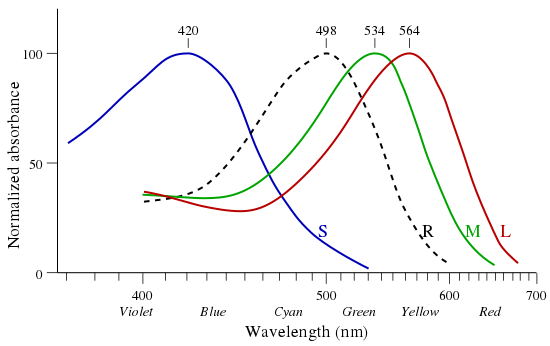
\includegraphics[width=8cm]{image/5-8-1.png}
\caption{四钟感光细胞约化吸收率}\label{fig:phtsens}
\end{wrapfigure}
大部分人类的视网膜内有两种大类的视觉感受细胞\footnote{还有\emph{内在光敏视网膜神经节细胞}(intrinsically photosensitive retinal ganglion cells, ipRGCs), 它含有\emph{视黑素}(melanopsin), 无法造成成像视觉, 但是在调节人昼夜节律方面发挥了主要功能.}:\,\emph{视锥细胞}(cone)与\emph{视杆细胞}(rod). 而视锥细胞又根据其所含视蛋白质分为感受$500-700\mathrm{nm}$波长的\emph{视红素}细胞(erythrolabe, L, $\rho$);\,感受$450-630\mathrm{nm}$波长的\emph{视绿素}细胞(chlorolabe, M, $\gamma$)和感受$400-500\mathrm{nm}$波长的\emph{视蓝素}细胞(cyanolabe, S, $\beta$)\footnote{在女性中常见异常X染色体导致个体产生四种色素的视锥细胞从而其色视觉明显优于一般的男性或女性}. 而视杆细胞由于结构差异导致比视锥细胞敏感约100倍, 单光子即可激发其\emph{视紫素}(rhodopsin, R)使其产生信号. 视紫素的合成需要依赖维生素A. 而维生素A的摄取除了动物性食物源还可以来自植物性植物中含有的$\beta$-胡萝卜素.

四种感光细胞对不同波长的光响应强度\ref{fig:phtsens}是不一致的. \emph{亮视觉}(photopic vision)才具有真正意义上的色视觉: 此时三种色素细胞L, M, S同时工作分管长, 中, 短波段的信号激励. 使得在可见光范围内的不同类似的光对三种色素细胞给出不同的激励值. 影响人对色彩的判断. 而在\emph{暗视觉}(scotopic vision)下前三种细胞失效, 视杆细胞积极发挥功能, 其视紫素R在$450-550\mathrm{nm}$波长范围有较强的吸收, 但是无法鉴别光的颜色. 所以暗视觉给人感觉接近灰度图, 同时红色物体在黑暗环境下比其它颜色物体更加昏暗. 这被称作\emph{浦金野现象}(Purkinje effect). 而有月光或星光的夜晚, 黎明与黄昏, 其实光线并没有暗到足够使得亮视觉失效. 此时的视觉称作\emph{中间视觉}(mesopic vision).

\begin{figure}[H]
\centering
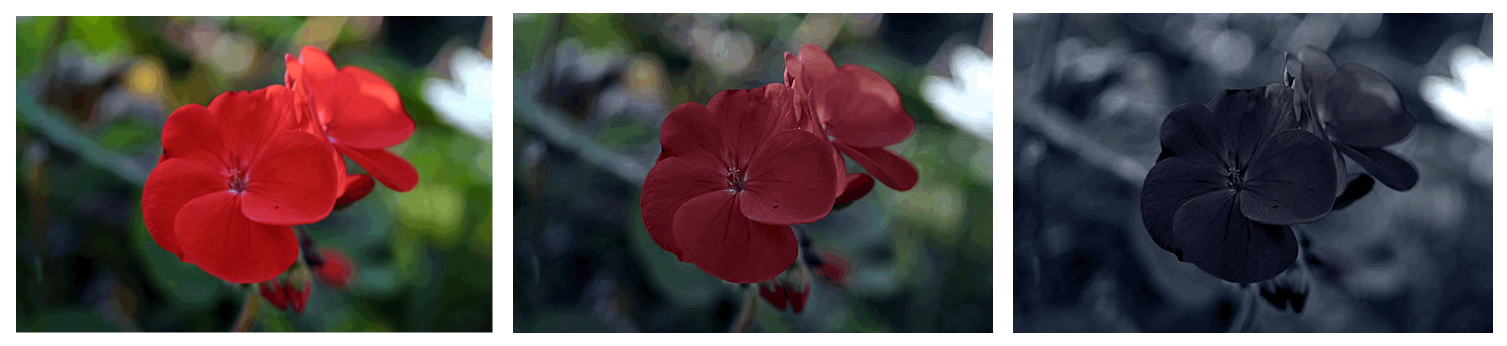
\includegraphics[width=16cm]{image/5-8-2.png}
\caption{浦金野现象}
\end{figure}

不同人的视觉条件当然存在区别. 粗的层面讲, 一束$555{\rm nm}$的位于人类视觉最敏感区的绿光和一束可见光边缘的$700{\rm nm}$的红光, 都给出$1{\rm W/m^2}$的平面波, 给人造成的亮度感觉一定是不一样的: 前者非常明亮而后者几乎不可见. 但是如果将一红一蓝两聚光灯聚焦于舞台再找两个人来比较哪个光斑更亮, 也许两个人就会给出不同的结果. 这种不同可能出于心理上或者生理上的效应. 但是如果要为照明制定标准, 就应该克服人与人之间的区别, 一般采取从大量受试者判断结果选取多数人的结果的方式. 这样就有了\emph{国际照明协会}(Commission Internationale de l\ap\'eclairage)在1931年通过的CIE1931标准. 它目前仍在广泛地被使用.

CIE1931标准将人眼中三种色素细胞的响应抽象为\emph{三激励值}(tristimulus values). 并将描述光的色彩, 亮度的空间抽象为\emph{色彩空间}(color space). 而色彩空间中的点就表示一种可能的色彩与亮度, 对应三激励值L, M, S, 构成一种加性空间: 三激励值的大小之和代表其明亮程度, 两组三激励值虽然组成不同但是和相等就说明. 如果以这三个参数建立坐标系表示色彩, 就称作LMS空间. 但是实用场合更常用的是$XYZ$空间. 它是这样定义的:

\begin{itemize}
\item $Y$定义为L, M, S的某种组合使得对不同单位强度的单色光其激励曲线与实际的总光强L+M+S曲线接近.
\item $Z$被直接定义为S值的某个倍数.
\item $X$定义为L, M, S的另一种组合使得对于所有的单色光其激励总是非负.
\end{itemize}






\section{光阑与光瞳}

\section{眼睛}

\section{显微镜}

\section{望远镜}

\section{照相机}